\section{Durchführung}
\label{sec:Durchführung}
\subsection{Zeitabhängigkeit der Amplitude}
Zunächst wird die Zeitabhängigkeit der Schwingungsamplitude untersucht.
Dazu wird der Versuch wie in Abbildung \ref{fig:aufbau1} aufgebaut und der Nadelimpulsgenerator so eingestellt, 
dass die Schwingung zwischen den Impulsen abklingen kann.
Um die Messung nicht mehr als nötig zu beeinflussen, wird für das Oszilloskop ein hochohmiger Tastkopf verwendet.
Es werden so viele Spitzen der abklingenden Schwingung wie möglich am Oszilloskop abgelesen.
\begin{figure}[H]
    \centering
    \caption{Versuchsaufbau für die Zeitabhängigkeit.\cite{v354}}
    \label{fig:aufbau1}
    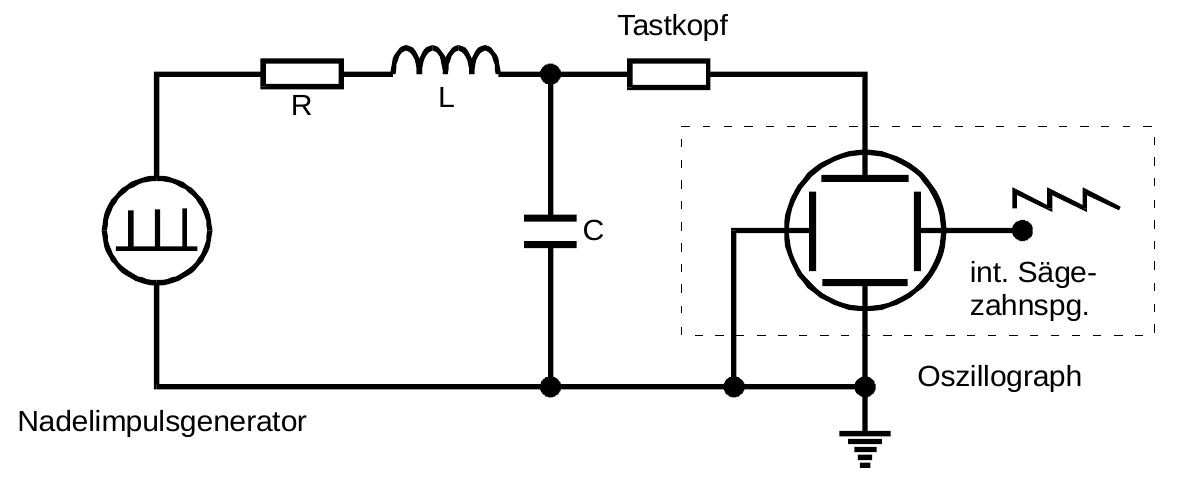
\includegraphics[width=\textwidth]{content/aufbau1.png}
\end{figure}
%
\subsection{Aperiodischer Grenzfall}
Die Messung wird ähnlich wie zuvor aufgebaut und ist in Abbildung \ref{fig:aufbau2} zu sehen.
Hierbei wird der Widerstand ermittelt, der bei einer gegebenen Apperatur einen apieriodischen Grenzfall hervorruft.
Dafür wird statt des festen Widerstandes ein Zehnerpotentiometer verwendet. 
Dieses wird aus einer hochohmigen Ausgangsposition solange geregelt, bis ein leichtes Überschwingen der Wellenform zu erkennen ist.
Anschließend wird das Potentiometer wieder ein kleines Stück zurückgeregelt, um wieder den Grenzfall zu erreichen.
\begin{figure}[H]
    \centering
    \caption{Versuchsaufbau für den aperiodischen Grenzfall.\cite{v354}}
    \label{fig:aufbau2}
    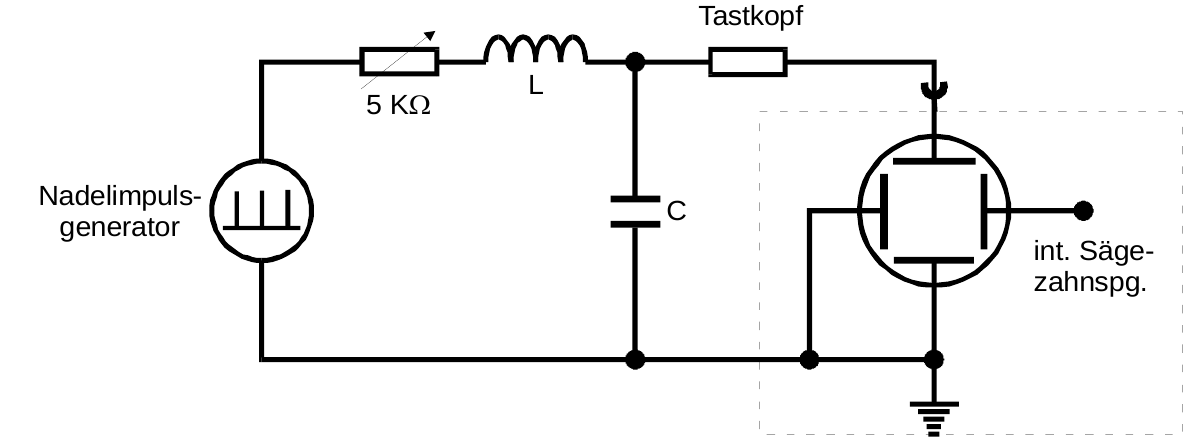
\includegraphics[width=\textwidth]{content/aufbau2.png}
\end{figure}
%
\subsection{Frequenzabhängigkeit der Amplitude}
Der Versuch wird ähnlich wie zuvor aufgebaut und ist in Abbildung \ref{fig:aufbau3} dargestellt.
Im Gegensatz zu den vorausgegangenen Messungen wird der Schwingkreis nun mit einem sinusförmigen Signal angeregt.
Damit wird über mehrere Zehnerpotenzen die resultierende Amplitude der Kondensatorspannung gemessen.
Hierbei ist darauf zu achten, dass auch der Tastkopf eine Impedanz besitzt und somit muss gleichzeitig die Quellspannung des Sinusgenerators gemessen werden.
\begin{figure}[H]
    \centering
    \caption{Versuchsaufbau für die frequenzabhängigkeit der Amplitude.\cite{v354}}
    \label{fig:aufbau3}
    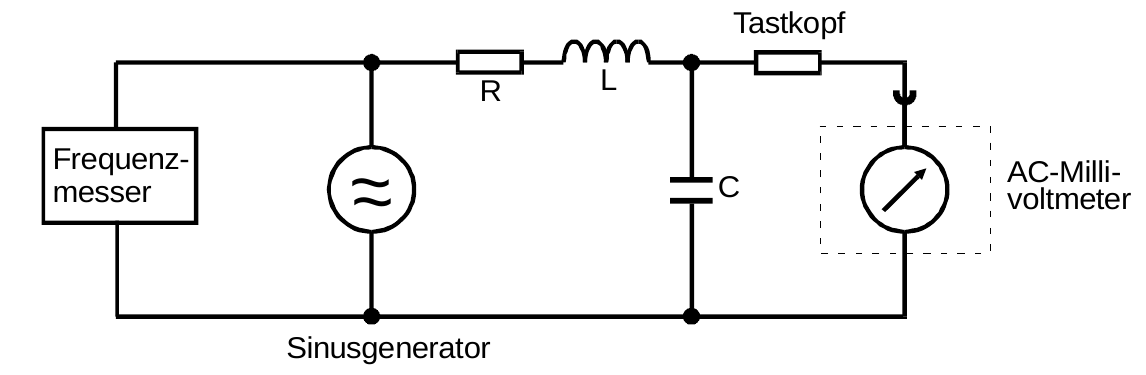
\includegraphics[width=\textwidth]{content/aufbau3.png}
\end{figure}
%
\subsection{Frequenzabhängigkeit des Phasenwinkels}
Dieser Aufbau ist nahe am vorausgegangenen, jedoch wird nun auf die Phasenverschiebung zwischen der Quellspannung und der Kondensatorspannung geachtet.
Dazu wird einerseits die zeitliche Verschiebung der Signale und die gesamte Periodendauer gemessen.
Auch hier findet die Messung über mehrere Zehnerpotenzen hinweg statt, 
wobei es ausreicht den Bereich um die Resonanzfrequenz zu betrachten.
Das Aufbauschume ist in Abbildung \ref{fig:aufbau4} zu sehen.
\begin{figure}[H]
    \centering
    \caption{Versuchsaufbau für die frequenzabhängigkeit der Phase.\cite{v354}}
    \label{fig:aufbau4}
    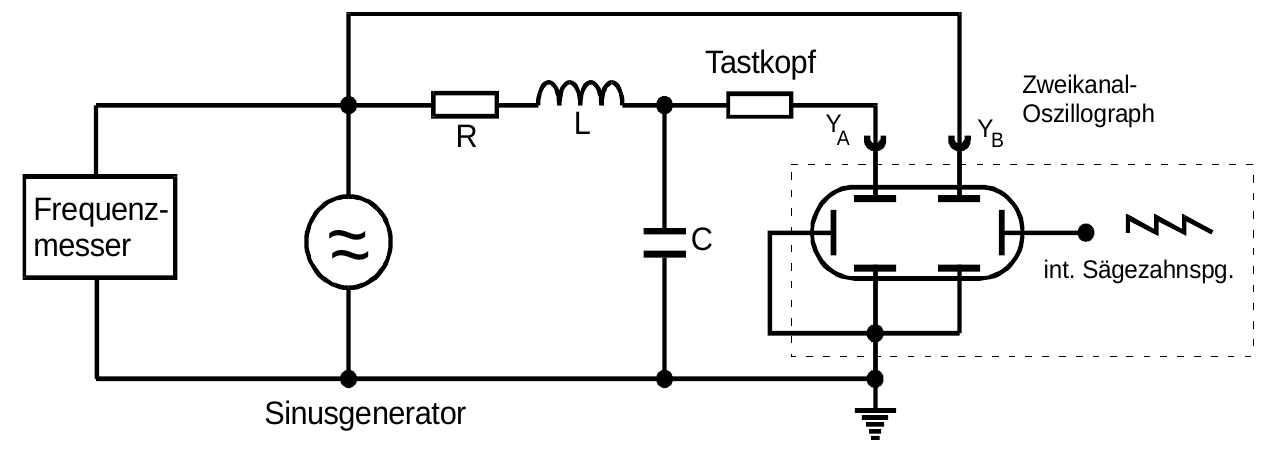
\includegraphics[width=\textwidth]{content/aufbau4.png}
\end{figure}
%
